\section*{1.}
\subsection*{a)}
\begin{itemize}[leftmargin=*]
  \item[] \(f(x,y) = e^{2 \pi i (px + qy)}\)

  \item[] Replace x with x(t) and y with y(t).\\
    \(g(t) = f(x(t),y(t)) = e^{2 \pi i (p (x_0 + tu_1) + q (y_0 + tu_2))}\)

  \item[] Multiply in p and q.\\
    \(= e^{2 \pi i (px_0 + ptu_1 + qy_0 + qtu_2)}\)

  \item[] Group \(p x_0\) with \(q y_0\), \(p u_1\) with \(q u_2\) and move \(t\) outside.\\
    \(= e^{2 \pi i ((px_0 + qy_0) + (pu_1 + qu_2) t)}\)

  \item[] Multiply in \(2 \pi i\)\\
    \(= e^{2 \pi i (px_0 + qy_0) + 2 \pi i (pu_1 + qu_2) t}\)

  \item[] \(v = (p,q)\), so replace \(q\) and \(p\) with \(v_1\) and \(v_2\) respectively.\\
    \(= e^{2 \pi i (px_0 + qy_0) + 2 \pi i (v_1 u_1 + v_2 u_2) t}\)

  \item[] Dot product is defined (for 2D vectors) as \(v \cdot w = v_1 w_1 + v_2 w_2\), so replace \((v_1 u_1 + v_2 u_2)\) with \((v \cdot u)\).\\
    \(= e^{2 \pi i (px_0 + qy_0) + 2 \pi i (v \cdot u) t}\)

  \item[] Dot product can be expanded to \(\norm{v} \norm{u} cos(\theta)\), so replace the dot product with it. \(\norm{u} = 1\), so we can remove it from the calculation.\\
    \(= e^{2 \pi i (px_0 + qy_0) + 2 \pi i (\norm{v} cos(\theta)) t}\)

  \item[] Split into two exponential functions: \(e^{x + y} = e^x e^y\).\\
    \(= e^{2 \pi i (px_0 + qy_0)} e^{2 \pi i(\norm{v} cos(\theta)) t}\)

  \item[] Set \(A = e^{2 \pi i (px_0 + qy_0)}\) since, as defined by the task, \say{\(A\) is some complex number that does not depend on t}.\\
    \(= A e^{2 \pi i (\norm{v} cos(\theta)) t}\)
\end{itemize}

\subsection*{b)}
When \(L\) is orthogonal to \(v\), \(u\) is also orthogonal to \(v\) since \(L\) has direction \(u\).
As seen from the calculations below, if \(u\) is orthogonal to \(v\), then the angle angle between them, \(\theta\), is \(\frac{\pi}{2}\), which will result into \(0\) from \(cos(\theta)\).
This means that the exponent ends up as \(0\), and \(e^0 = 1\).
Only the constant \(A\) then remains.
See below for the steps.
\begin{itemize}[leftmargin=*]
  \item[] \(g(t) = A e^{2 \pi i (\norm{v} cos(\theta)) t}\)
  \item[] \(= A e^{2 \pi i (\norm{v} cos(\frac{\pi}{2})) t}\)
  \item[] \(= A e^{2 \pi i (\norm{v} 0) t}\)
  \item[] \(= A e^{0}\)
  \item[] \(= A\)
\end{itemize}

\subsection*{c)}


\begin{enumerate}
  \item \(A e^{2 \pi i (\norm{v} cos(\theta)) t}\)
  \item \(2 \pi i (\norm{v} cos(\theta)) t\)

    The exponent of \(e\) defines the frequency.
  \item \(2 \pi i (\norm{v} cos(\theta))\)

    Since the question is \say{per unit distance}, \(t = 1\) and we can remove it from the calculation.
  \item \(\norm{v} cos(\theta)\)

    \(2 \pi\) is one cycle (one oscillation), so the values that are multiplied with \(2 \pi\) is the frequency. Thus we can remove \(2 \pi\)
  \item \(\sqrt{p^2 + q^2} cos(\theta)\)

    \(\norm{v}\) is replaced by \(\sqrt{p^2 + q^2}\) since \(\norm{v} = \sqrt{v_1^2 + v_2^2}\) and \(v = (p,q)\). This is the frequencey in terms of \(p\), \(q\) and \(\theta\).
\end{enumerate}

\subsection*{d)}
The larger the exponent is, the larger the frequencey is, therefore the returned value from \(cos(\theta)\) must be as high as possible.
\(cos\) cycles from \(1\) to \(0\) to \(-1\) to \(0\) and back to \(1\).
From this it is obvious that \(1\) is the largest value.
To get \(1\) from \(cos\), the input must be \(0\) or \(0 + n 2 \pi\), where \(n\) is any integer.
This means that the value of \(\theta\) which maximizes the frequency is \(0\).

While \(\theta\) from b) was \(\frac{\pi}{2}\), this time it is \(0\).
Whit an angle of \(\frac{\pi}{2}\), \(u\) is orthogonal to \(v\).
Whit an angle of \(0\), \(u\) is parallel to \(v\) (same direction).
The resulting frequency from \(\theta = \frac{\pi}{2}\) will be \(0\), while it will now be the frequency defined below.

In terms of p and q, the maximum frequencey is \(\sqrt{p^2 + q^2}\), calculated from the list below.
When \(\theta\) is \(0\) (to maximize frequencey), \(cos(\theta)\) is 1, so we can eliminate it from the formula.
\begin{enumerate}
  \item \(\sqrt{p^2 + q^2} cos(\theta)\)
  \item \(\sqrt{p^2 + q^2} cos(0)\)
  \item \(\sqrt{p^2 + q^2} 1\)
  \item \(\sqrt{p^2 + q^2}\)
\end{enumerate}

\subsection*{e)}
The wavelength is calculated by \(\lambda = \frac{2 \pi}{\abs{\omega}}\).
Since \(f(x,y)\) is two-dimensional, it has a wavelength in both x and y direction:
\(e^{2 \pi i (p x + q y)} = e^{2 \pi i p x} e^{2 \pi i q y}\).
From \(e^{i \omega t}\) it is clear that \(\omega = p\) and \(\omega = q\).
Thus the frequencies are:
\begin{itemize}
  \item For x: \(\frac{2 \pi}{\abs{p}}\)
  \item For y: \(\frac{2 \pi}{\abs{q}}\)
\end{itemize}
By using the answer from 2d, the wavelength of \(g(t) = f(x(t),y(t))\) will be \(\frac{2 \pi}{\sqrt{p^2 + q^2}}\).

\section*{2.}
\subsection*{a)}
See 2a.py for the source code, and the figure below for the plot.

\begin{figure}[H]
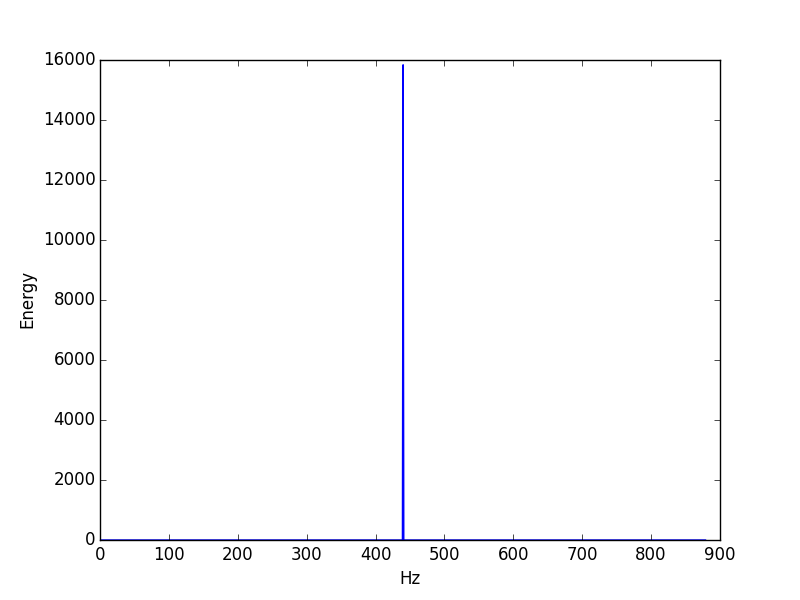
\includegraphics[width=\textwidth]{2a_power_spectrum}
\caption{Power spectrum}
\label{fig:2a}
\end{figure}

\subsection*{b)}
Calculation for \(x_1[n]\):
\begin{itemize}[leftmargin=*]
  \item[] \(X_0 = 1 e^{-2 \pi i 0 \cdot 0 / 4} + 1 e^{-2 \pi i 0 \cdot 1 / 4} + 1 e^{-2 \pi i 0 \cdot 2 / 4} + 1 e^{-2 \pi i 0 \cdot 3 / 4}\)
  \item[] \(= e^0 + e^0 + e^0 + e^0\)
  \item[] \(= 1 + 1 + 1 + 1\)
  \item[] \(= 4\)
\end{itemize}
\begin{itemize}[leftmargin=*]
  \item[] \(X_1 = 1 e^{-2 \pi i 1 \cdot 0 / 4} + 1 e^{-2 \pi i 1 \cdot 1 / 4} + 1 e^{-2 \pi i 1 \cdot 2 / 4} + 1 e^{-2 \pi i 1 \cdot 3 / 4}\)
  \item[] \(= e^0 + e^{-2 \pi i / 4} + e^{-4 \pi i / 4} + e^{-6 \pi i / 4}\)
  \item[] \(= 1 + -i + (-1) + i\)
  \item[] \(= 0\)
\end{itemize}
\begin{itemize}[leftmargin=*]
  \item[] \(X_2 = 1 e^{-2 \pi i 2 \cdot 0 / 4} + 1 e^{-2 \pi i 2 \cdot 1 / 4} + 1 e^{-2 \pi i 2 \cdot 2 / 4} + 1 e^{-2 \pi i 2 \cdot 3 / 4}\)
  \item[] \(= e^0 + e^{-4 \pi i / 4} + e^{-8 \pi i / 4} + e^{-12 \pi i / 4}\)
  \item[] \(= 1 + (-1) + 1 + (-1)\)
  \item[] \(= 0\)
\end{itemize}
\begin{itemize}[leftmargin=*]
  \item[] \(X_3 = 1 e^{-2 \pi i 3 \cdot 0 / 4} + 1 e^{-2 \pi i 3 \cdot 1 / 4} + 1 e^{-2 \pi i 3 \cdot 2 / 4} + 1 e^{-2 \pi i 3 \cdot 3 / 4}\)
  \item[] \(= e^0 + e^{-3 \pi i / 4} + e^{-6 \pi i / 4} + e^{-18 \pi i / 4}\)
  \item[] \(= 1 + i + (-1) + -i\)
  \item[] \(= 0\)
\end{itemize}
For \(x_2[n]\) and \(x_3[n]\), the 0's will cancel out the calulation of that index, meaning that they won't have any effect on the dft.
Thus the calculated spectrums are exactly the same.
See 2b.py for the source code, and the figures below for the plots.

\begin{figure}[H]
  \centering
  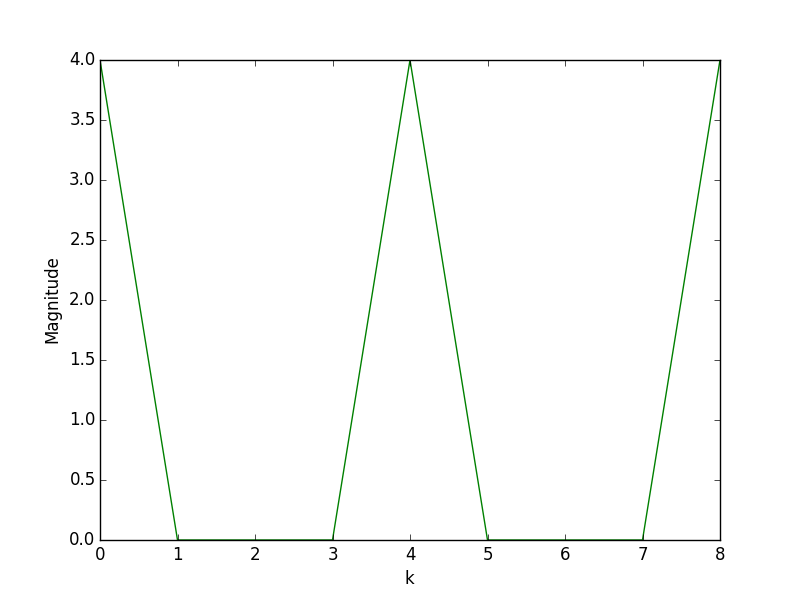
\includegraphics[width=\linewidth]{2b_1}
  \caption{x1[n]}
  \label{fig:2b1}
\end{figure}
\begin{figure}[H]
  \centering
  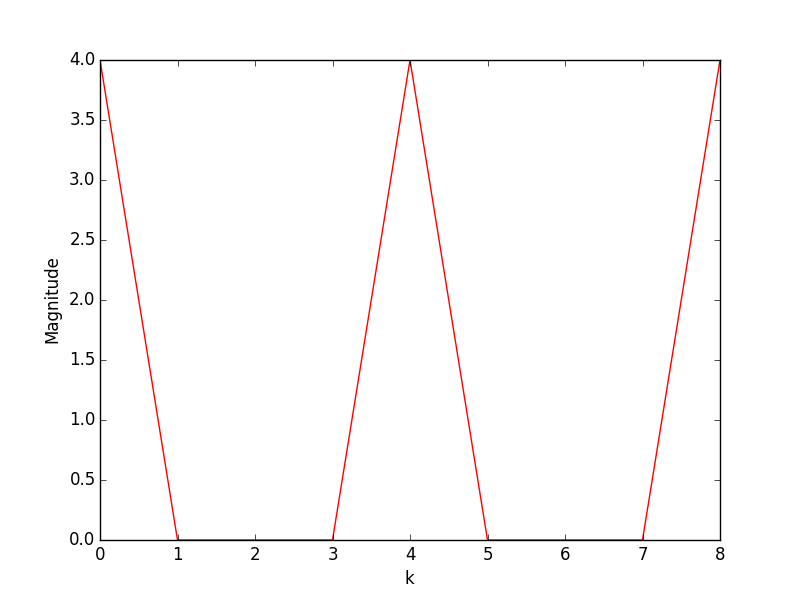
\includegraphics[width=\linewidth]{2b_2}
  \caption{x2[n]}
  \label{fig:2b2}
\end{figure}
\begin{figure}[H]
  \centering
  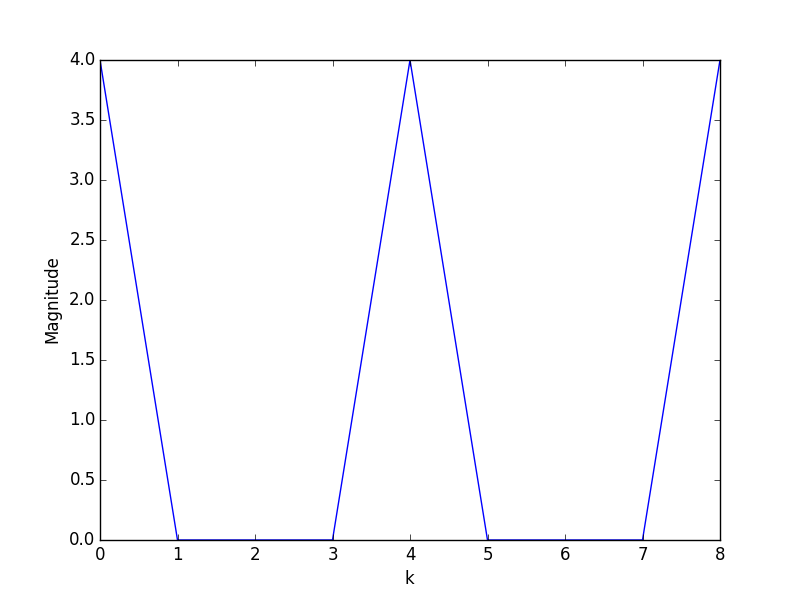
\includegraphics[width=\linewidth]{2b_3}
  \caption{x3[n]}
  \label{fig:2b3}
\end{figure}

\subsection*{c)}
\subsubsection*{i)}
\begin{itemize}[leftmargin=*]
  \item[] \(X_k = \displaystyle\sum_{n = 0}^{N - 1} x_n e^{-2 \pi i k n / N}\)
  \item[] \(X_1[k] = \displaystyle\sum_{n = 0}^{N - 1} x_1[n] e^{-2 \pi i k n / N}\)
  \item[] \(= \displaystyle\sum_{n = 0}^{N - 1} x[n] cos(2 \pi n m / N) e^{-2 \pi i k n / N}\)
\end{itemize}

\subsubsection*{ii)}
\begin{itemize}[leftmargin=*]
  \item[] \(X_k = \displaystyle\sum_{n = 0}^{N - 1} x_n e^{-2 \pi i k n / N}\)
  \item[] \(X_2[k] = \displaystyle\sum_{n = 0}^{N - 1} x_2[n] e^{-2 \pi i k n / N}\)
  \item[] \(= \displaystyle\sum_{n = 0}^{N - 1} x[n] sin(2 \pi n m / N) e^{-2 \pi i k n / N}\)
\end{itemize}

\subsection*{d)}
\subsubsection*{i)}
The samples for 4hz are as follows.
\begin{itemize}[leftmargin=*]
  \item[] \(x(t) = sin(2 \pi t)\)
  \item[] \(x(0) = sin(0) = 0\)
  \item[] \(x(\frac{1}{4}) = sin(\frac{\pi}{2}) = 1\)
  \item[] \(x(\frac{2}{4}) = sin(\pi) = 0\)
  \item[] \(x(\frac{3}{4}) = sin(\frac{3 \pi}{2}) = -1\)
\end{itemize}
\(x = (0, 1, 0, -1)\)\\\\
The \(c_k\)'s are as follows.
\begin{itemize}[leftmargin=*]
  \item[] \(c_0 = \frac{1}{4} (1 e^{-2 \pi i 0 \cdot 0 / 4} + 0 e^{-2 \pi i 0 \cdot 1 / 4} -1 e^{-2 \pi i 0 \cdot 2 / 4} + 0 e^{-2 \pi i 0 \cdot 3 / 4})\)
  \item[] \(= \frac{1}{4} (e^0 - e^0)\)
  \item[] \(= \frac{1}{4} (1 - 1)\)
  \item[] \(= 0\)
\end{itemize}
\begin{itemize}[leftmargin=*]
  \item[] \(c_1 = \frac{1}{4} (0 e^{-2 \pi i 1 \cdot 0 / 4} + 1 e^{-2 \pi i 1 \cdot 1 / 4} + 0 e^{-2 \pi i 1 \cdot 2 / 4} - 1 e^{-2 \pi i 1 \cdot 3 / 4})\)
  \item[] \(= \frac{1}{4} (e^{-\pi i / 2} - e^{-3 \pi i / 2})\)
  \item[] \(= \frac{1}{4} (-i - i)\)
  \item[] \(= -\frac{i}{2}\)
\end{itemize}
\begin{itemize}[leftmargin=*]
  \item[] \(c_2 = \frac{1}{4} (0 e^{-2 \pi i 2 \cdot 0 / 4} + 1 e^{-2 \pi i 2 \cdot 1 / 4} + 0 e^{-2 \pi i 2 \cdot 2 / 4} + -1 e^{-2 \pi i 2 \cdot 3 / 4})\)
  \item[] \(= \frac{1}{4} (e^{-\pi i} - e^{-3 \pi i})\)
  \item[] \(= \frac{1}{4} (-1 - (-1))\)
  \item[] \(= 0\)
\end{itemize}
\begin{itemize}[leftmargin=*]
  \item[] \(c_3 = \frac{1}{4} (0 e^{-2 \pi i 3 \cdot 0 / 4} + 1 e^{-2 \pi i 3 \cdot 1 / 4} + 0 e^{-2 \pi i 3 \cdot 2 / 4} - 1 e^{-2 \pi i 3 \cdot 3 / 4})\)
  \item[] \(= \frac{1}{4} (e^{-3 \pi i / 2} - e^{-9 \pi i / 2})\)
  \item[] \(= \frac{1}{4} (i - (-i))\)
  \item[] \(= \frac{i}{2}\)
\end{itemize}
\(c = (0, -0.5i, 0, 0.5i)\)

\subsubsection*{ii)}
See 2d.py for the source code.
\begin{figure}[H]
  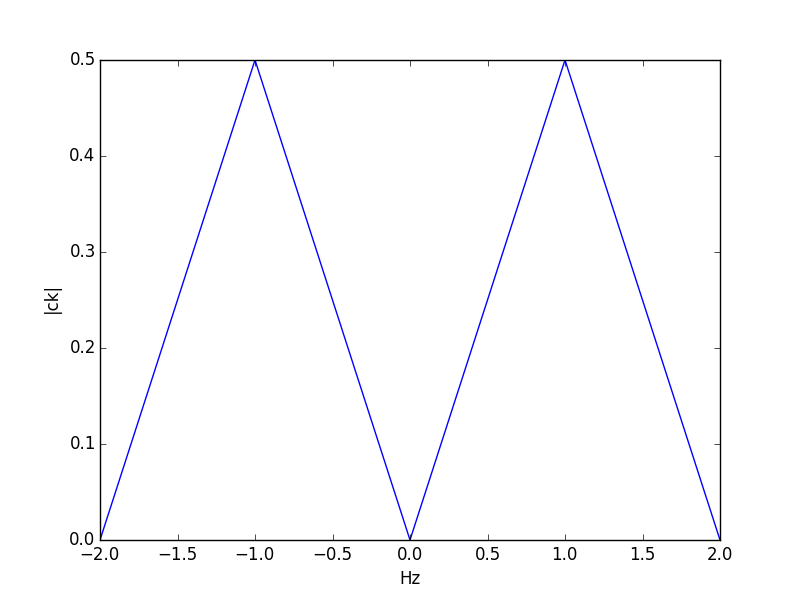
\includegraphics[width=\textwidth]{2dii}
  \caption{spectrum over [-2hz,2hz]}
  \label{fig:2dii}
\end{figure}

% vim: set ts=2 sw=2 expandtab:
